\documentclass[aspectratio=169,
				xcolor=table]{beamer}

% Load general definitions
\usepackage[utf8]{inputenc}
%\usepackage[T1]{fontenc}
\usepackage[brazil]{babel}
\usepackage{amsmath}
\usepackage{amsfonts}
\usepackage{amssymb}
\usepackage{graphicx}
\usepackage{verbatim}
\usepackage{cancel}
\usepackage{askmaps}
\usepackage{tabularx}
\usepackage[table]{xcolor}
%\usepackage{tikz}
\usepackage{multirow}
\usepackage{mathtools}
\usepackage{color, colortbl}
\usepackage{etoolbox}
\usepackage{pbox}
\usepackage{changepage}
\usepackage{xpatch}
\usepackage{array}
\usepackage{marvosym}
\usepackage{tabu}
\usepackage{multicol}
\usepackage{listings}
\usepackage{underscore}
\usepackage{filecontents}
\usepackage[]{algorithm2e}
\usepackage{ragged2e}

\newcolumntype{P}[1]{>{\centering\arraybackslash}m{#1}}
\definecolor{Gray}{gray}{0.75}
\definecolor{Gray2}{gray}{0.85}

\definecolor{lightBlue}{HTML}{DAE8FC}
\definecolor{Blue}{RGB}{51, 51, 204}

%\useinnertheme[lily]{rounded}
\usetheme{UniEvangelica}
%\usetheme{Copenhagen}
%\usetheme{Berlin}
%\usecolortheme{dolphin}
\tolerance=1
\emergencystretch=\maxdimen
\hyphenpenalty=10000
\hbadness=10000

\setbeamertemplate{navigation symbols}{}%remove navigation symbols


\let\olditem=\item% 
\renewcommand{\item}{\olditem \justifying}%
\def\center{\trivlist \centering\item\relax}
\def\endcenter{\endtrivlist}

\setbeamertemplate{itemize/enumerate body begin}{\large}
\setbeamertemplate{itemize/enumerate subbody begin}{\large}

\setbeamertemplate{itemize item}{\raisebox{0.1ex}{$\blacktriangleright$}\hskip0.1em}
\setbeamertemplate{itemize subitem}{\raisebox{0.1ex}{$\blacktriangleright$}\hskip0.1em}

\newcommand{\greenarrow}{\textcolor{green}{\rotatebox[origin=c]{180}{\MVArrowDown}}}

\newcommand{\redarrow}{\textcolor{red}{\MVArrowDown}}

%\newcommand{\ftable}{
%	\begin{table}
%		\large
%		\centering
%		\rowcolors{1}{\ifnumless{\rownum}{2}{Blue}{lightBlue}}{}
%}

\newenvironment{eftable}{
	\begin{table}
		\large
		\centering
		\rowcolors{1}{}{Blue}
		\rowcolors{1}{\ifnumless{\rownum}{2}{Blue}{lightBlue}}{}
	}
	{
	\end{table}
}


%\setbeamertemplate{frametitle}
%{
%	%\vspace*{-2em}	
%	\insertframetitle
%
%	 %\textcolor{white}{\LARGE \insertframetitle}
%
%}

% Specific definitions
\institute[]{\uppercase{Engenharia de Software}}
\title[]{Sistemas Operacionais}
\subtitle[]{Escalonamento de Processos }
\author[]{Prof. M.e Alexandre Tannus}
\date{Anápolis - 2021.1}

\AtBeginSection{\frame{\tableofcontents[currentsection]}}

\begin{document}
	\begin{frame}
		\titlepage
	\end{frame}

	\begin{frame}
		\tableofcontents
	\end{frame}	
	
	
	\begin{frame}{Questionamentos}
		\begin{itemize}
			\item Como o sistema operacional escolhe os processos para execução?
			\vspace{1em}
			\item Quais algoritmos podem ser utilizados?
			\vspace{1em}
			\item Quais impactos cada algoritmo pode trazer para o desempenho geral do sistema?
		\end{itemize}
	\end{frame}

	\section{Introdução}
	\begin{frame}{Relembrando - Transições de Estado}		
		\begin{figure}[hbtp]
			\centering
			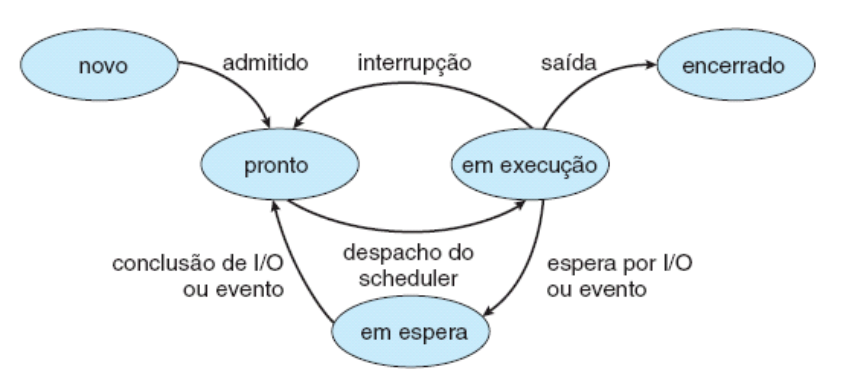
\includegraphics[keepaspectratio, width=.9\textwidth]{../figs/cap03/estados.png}	
		\end{figure} 
	\end{frame}	
	
	\begin{frame}{Relembrando - Estrutura do processo}	
		\begin{figure}[hbtp]
		\centering
		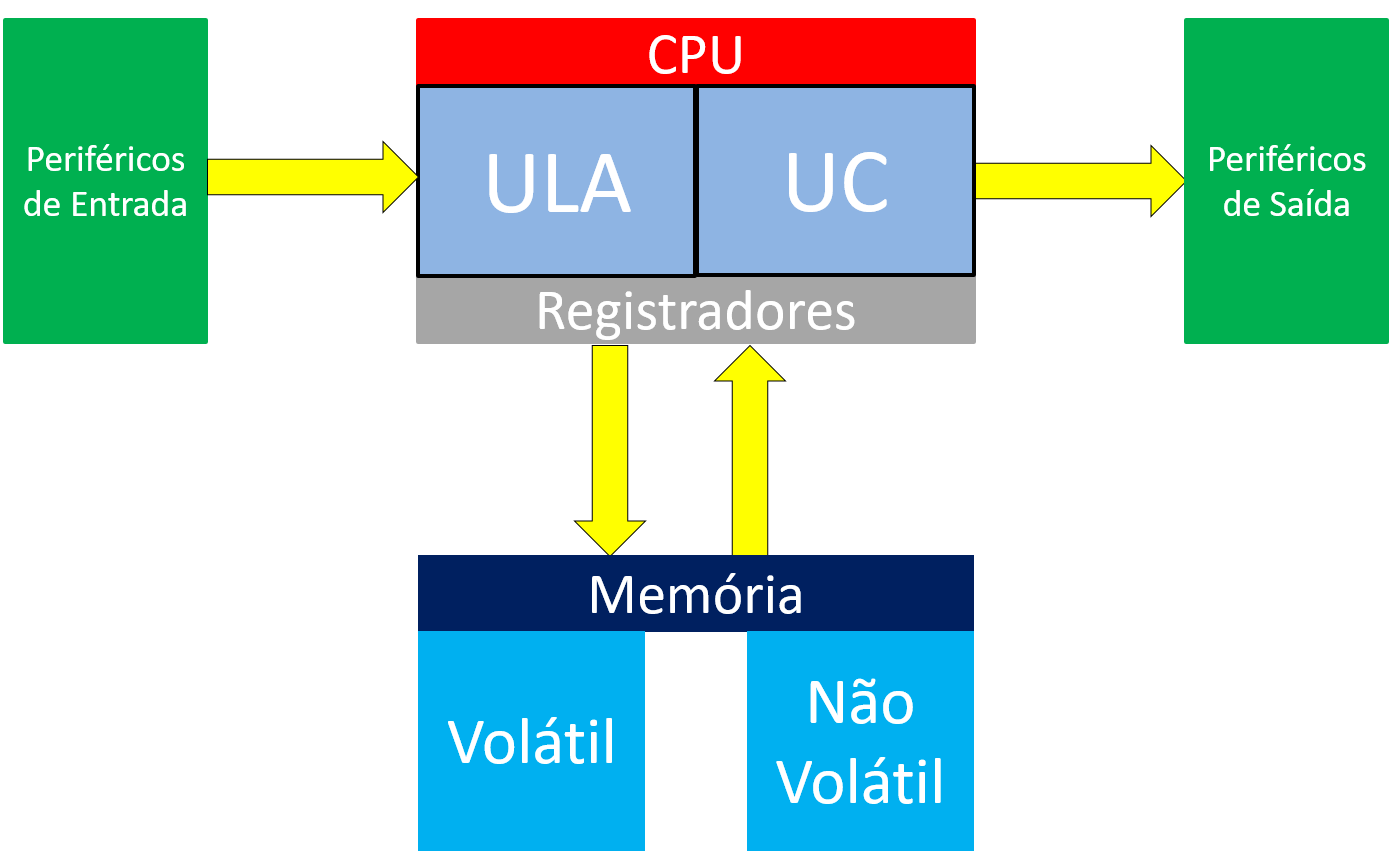
\includegraphics[keepaspectratio, height=.8\textheight]{../figs/cap03/estrutura.png}
		\end{figure}
	\end{frame}	
	
	\begin{frame}{Relembrando - Estrutura de \textit{thread}}
		\begin{figure}[hbtp]
			\centering
			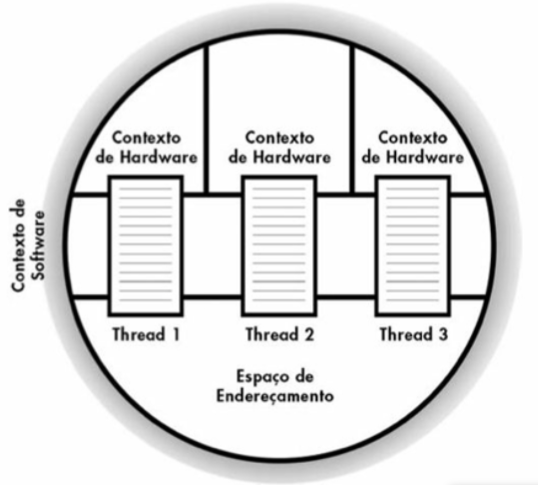
\includegraphics[height=.85\textheight, keepaspectratio]{../figs/cap04/multithread02.png}
		\end{figure}	
	\end{frame}	
	
	\begin{frame}{Relembrando - Troca de Contexto}
		\begin{figure}[hbtp]
			\centering
			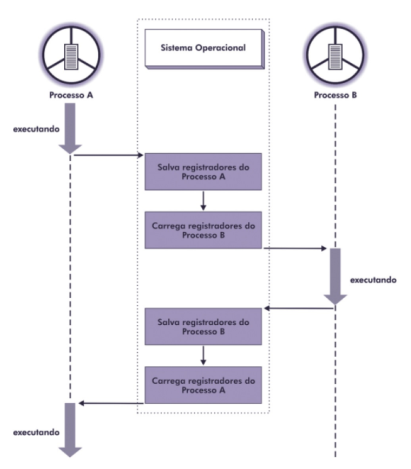
\includegraphics[keepaspectratio, height=.8\textheight]{../figs/cap03/contextohard.png}
		\end{figure}
	\end{frame}
	
	\begin{frame}{Escalonamento de Processos}
		\begin{itemize}
			\item Sistemas monoprocessados
			\begin{itemize}
			 	\item Execução de um processo por vez
			 	\item Outros processos devem aguardar a liberação da CPU
			 	\item \alert{Problema: desperdício de uso da CPU}
			 \end{itemize} 
			 \vspace{1em}
			 \item Multiprogramação
			 \begin{itemize}
			 	\item Possibilidade de aumentar a eficiência no uso da CPU
			 \end{itemize}
		\end{itemize}
	\end{frame}	
	
	\begin{frame}{Escalonamento de Processos}
		\begin{itemize}
			\item Escalonador
			\begin{itemize}
				\item Parte do sistema operacional responsável pela escolha do processo que será executado em um dado momento.
				\item Seleciona um processo na lista de \textit{Pronto} e aloca a CPU a esse processo
			\end{itemize}
			\vspace{1em}
			\item Algoritmo de escalonamento
			\begin{itemize}
				\item Método utilizado pelo sistema operacional para realizar a escolha
			\end{itemize}
		\end{itemize}
	\end{frame}
	
	\begin{frame}{Quando escalonar um processo?}
		\begin{enumerate}
			\item Quando um novo processo é criado.
			\vspace{0.75em}
			\item Quando ocorre uma interrupção.
			\vspace{0.75em}		
			\item Quando um processo é bloqueado por uma operação de E/S.
			\vspace{0.75em}
			\item Quando um processo termina.			
		\end{enumerate}
	\end{frame}
		
	\begin{frame}{Formas de escalonamento}
		\begin{itemize}
			\item Não Preemptivo
			\begin{itemize}
				\item Execução de um processo selecionado até
				\begin{itemize}
					\item Finalização do processo
					\item Bloqueio do processo por E/S
					\item Liberação voluntária da CPU pelo processo
				\end{itemize}
			\end{itemize}
			\vspace{1em}			
			\item Preemptivo
			\begin{itemize}
				\item Execução de um processo selecionado por um tempo fixo
				\item Suspensão do processo ao final do tempo e seleção de outro processo para execução
			\end{itemize}
		\end{itemize}		
	\end{frame}
	
	\begin{frame}{Despachante (\textit{dispatcher})}
		\begin{itemize}
			\item Módulo que passa o controle da CPU ao processo selecionado pelo escalonador
			\vspace{1em}
			\item Responsável pela troca de contexto
			\vspace{1em}
			\item Latência do despacho
			\begin{itemize}
				\item Tempo necessário para interrupção de um processo e inicialização de outro processo
				\item Deve ser o mais rápido possível
			\end{itemize}
		\end{itemize}			
	\end{frame}	
	
	\begin{frame}{Objetivos - Todos os sistemas}
		\begin{itemize}
			\item Imparcialidade
			\begin{itemize}
				\item Todo processo recebe o mesmo tempo de CPU
			\end{itemize}
			\vspace{1em}
			\item Imposição da política
			\begin{itemize}
				\item Garantir a execução da política 
			\end{itemize}
			\vspace{1em}
			\item Balanceamento de carga					
			\begin{itemize}
				\item Manter a ocupação de todas as partes do sistema
			\end{itemize}
		\end{itemize}
	\end{frame}
	
	\begin{frame}{Objetivos - Sistemas de lotes}
		\begin{itemize}
			\item Taxa de saída (\textit{throughput})
			\begin{itemize}
				\item Maximização do número de \textit{jobs} por unidade de tempo
			\end{itemize}
			\vspace{1em}
			\item Tempo de retorno (\textit{turnaround})
			\begin{itemize}
				\item Minimizar tempo entre envio e término de uma tarefa
			\end{itemize}
			\vspace{1em}
			\item Utilização da CPU
			\begin{itemize}
				\item Otimização do tempo de uso da CPU
			\end{itemize}
		\end{itemize}
	\end{frame}
		
	\begin{frame}{Objetivos - Sistemas interativos}
		\begin{itemize}
			\item Tempo de resposta
			\begin{itemize}
				\item Rápido atendimento das requisições
			\end{itemize}
			\vspace{1em}
			\item Proporcionalidade
			\begin{itemize}
				\item Atender às expectativas dos usuários
			\end{itemize}
		\end{itemize}
	\end{frame}
		
	\begin{frame}{Objetivos - Sistemas de tempo real}
		\begin{itemize}
			\item Cumprimento de prazos
			\begin{itemize}
				\item Evitar perda de dados
			\end{itemize}
			\vspace{1em}
			\item Previsibilidade
			\begin{itemize}
				\item Evitar degradação de qualidade
			\end{itemize}
		\end{itemize}
	\end{frame}
	
	\section{Algoritmos de Escalonamento}
	\begin{frame}{Algoritmos de Escalonamento}
		\begin{itemize}
			\item Primeiro a chegar, primeiro a ser servido (\textit{First Come, First Served} - FCFS)
			\item Tarefa mais curta primeiro (\textit{Shortest Job First} - SJF)
			\item Por prioridades
			\item \textit{Round Robin}
			\item Filas Multiníveis
		\end{itemize}
	\end{frame}
	
	\begin{frame}{\textit{First Come, First Served} - FCFS}
		\begin{itemize}
			\item Algoritmo não preemptivo 
			\vspace{1em}
			\item Processo que solicita a CPU primeiro será executado primeiro			
		\end{itemize}
		\begin{figure}[hbtp]
		\centering
		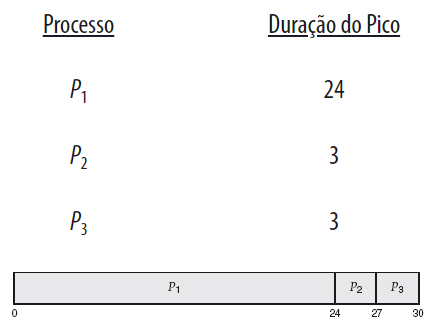
\includegraphics[keepaspectratio, height=.6\textheight]{../figs/cap06/fcfs.png}
		\end{figure}				
	\end{frame}
	
	\begin{frame}{\textit{Shortest Job First} - SJF}
		\begin{itemize}
			\item Algoritmo não preemptivo 
			\vspace{1em}
			\item Seleciona o processo com tempo de execução mais curto para ser executado
						
		\end{itemize}
		\begin{figure}[hbtp]
		\centering
		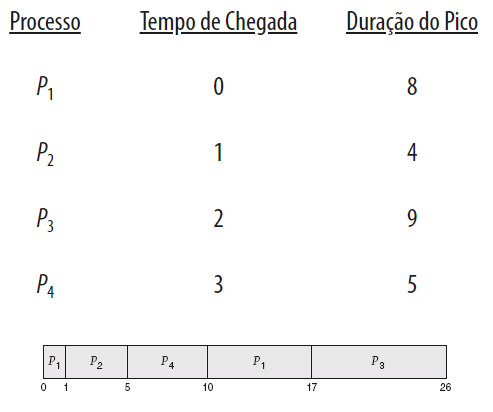
\includegraphics[keepaspectratio, height=.6\textheight]{../figs/cap06/sjf.png}
		\end{figure}			
	\end{frame}

	
	\begin{frame}{Escalonamento por Prioridade}
		\begin{itemize}
			\item Algoritmo não preemptivo 
			\vspace{0.5em}
			\item Seleciona o processo com base em prioridades estabelecidas
			\vspace{0.5em}
			\item Prioridades podem ser estáticas ou dinâmicas
						
		\end{itemize}
		\begin{figure}[hbtp]
		\centering
		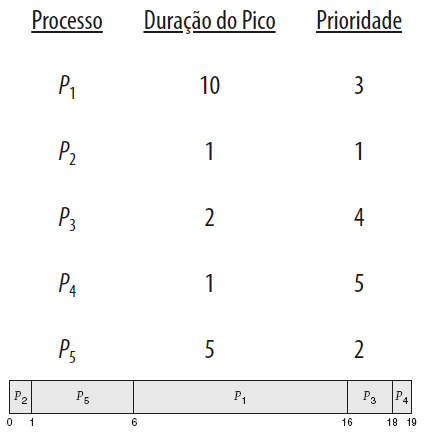
\includegraphics[keepaspectratio, height=.6\textheight]{../figs/cap06/prioridade.png}
		\end{figure}			
	\end{frame}		
			
	\begin{frame}{\textit{Round Robin}}
		\begin{itemize}
			\item Algoritmo preemptivo 
			\vspace{1em}
			\item Similar ao FCFS, mas com tempo limitado para cada processo (\textit{quantum})	
						
		\end{itemize}
		\begin{figure}[hbtp]
		\centering
		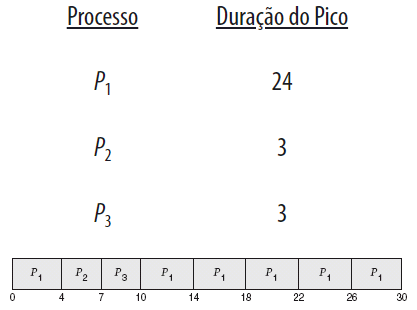
\includegraphics[keepaspectratio, height=.6\textheight]{../figs/cap06/rr.png}
		\end{figure}			
	\end{frame}	
	
	\begin{frame}{Impacto do \textit{quantum} de tempo}
		\begin{figure}[hbtp]
		\centering
		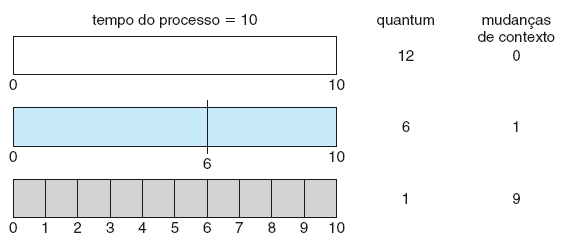
\includegraphics[keepaspectratio, height=.6\textheight]{../figs/cap06/quantum.png}
		\end{figure}					
	\end{frame}	
	
	\begin{frame}{Bibliografia}
		\begin{itemize}
			\item SILBERSCHATZ, A.; GALVIN, P. B.; GAGNE, G.. \textbf{Fundamentos de sistemas operacionais: princípios básicos.} Rio de Janeiro: LTC – Livros Técnicos e Científicos, 2013.
			
			\vspace{1em}

			\item TANENBAUM, A.S., WOODHULL, A.S. \textbf{Sistemas Operacionais.} Porto Alegre: Grupo A, 2008.
			
		\end{itemize}
	\end{frame}


	\begin{frame}{}
	\end{frame}	
	
\end{document}
